\documentclass[
	aspectratio=169,	% Modern aspect ratio (TODO: Other ratios not yet supported)
	onlytextwidth,		% Sets totalwidth=\textwidth and therefore e.g. columns won't invade the margins
	t,					% Default vertical alignment of frames and colums at top (default is centered) % Stored in \beamer@centered (\beamer@centeredfalse, \beamer@centeredtrue)
%	handout,			% Create a basic handout of the presentation (removes overlays)
	]{beamer}

%%%%%%%%%%%%%%%%%%%%%%%%%%%%%%%%%%%%%%%%%%
% 1) Load the desired presentation theme
\usetheme[
% Individual options to customize the presentation conforming to the corporate design
	hs,					% Change default faculty color set and predefined faculty values: hs or <empty> (default), inw, cb, me, sw, wi, inst (\renewcommand{\insertfacultyname}{Institutname} needed)
	language=english,	% Change language to english (default: ngerman), other languages are possible (see babel-package) but may need further adjustments 
	toc,				% Adds a ToC slide
	sectionslide,		% Display separate section slides
	subsectionslide,		% Display separate subsection slides containing section and subsection name
%	smallpagenumber,	% Reduces the size of the page number
%	nototalpages,		% Hides the total number of slide in footline
%	nofacultyicon,		% Hides the faculty icon on title page
	colormath=nottext,	% Enables coloring of math text: off or <empty>, full, nottext (default)
%	printhandout,		% Places two slides on a single a4 paper for printing the presentation (beamer class option 'handout' needed)
%	noframesubtitle,	% Disables frame subtitles alltogether and slightly increases frame height
% Additional style options not completely conforming to the corporate design
	titlepagedate,		% Shows the date on the titelpage
%	fancystyle,			% Enables some fancy styles, that are not part of the corporate design specifications (default: off)
%	progressbar,		% Shows the progressbar in footline (run twice to update progressbar)
	]{hsmw} 

%%%%%%%%%%%%%%%%%%%%%%%%%%%%%%%%%%%%%%%%%%
% 2) Specify default fields for presentation and pdf document properties
% Set the title: \title{Long title everywhere} or \title[Short title for footline]{Long title for titlepage}
\title[Cognitive Science and Machine Learning]{Cognitive Science and Machine Learning}
\subtitle{}
% Authors (separate multiple author names e.g. with \and for additional space): \author{author for everywhere} or \author[author for footline]{author for titlepage and thankyouslide}
\author[Mert Saruhan]{Mert Saruhan, B.Sc.}
% Institute (will be prefilled automatically, depending on chosen faculty theme option): \institute{institute for everywhere} or \institute[institute for footline and thankyouslide]{institute for titlepage}
%\institute[Fakultät Angewandte Computer und Biowissenschaften]{Fakultät Angewandte Computer und Biowissenschaften}
% Date of presentation (\today or a fixed value): \date{date for everywhere} or \date[date for footline]{date for titlepage}
\date{\today} % 22. März 2022
% Impressum for thankyou slide (leave one empty if not wanted or needed):
\email{msaruhan@hs-mittweida.de} % \email{E-Mail}
\courseofstudies{Mathematics for Network and Data Science (MA20w1-M)} % \courseofstudies{Course of Studies (Group Number)}
%\additional[Sidebar Text]{Main Text} % Additional information you may want to give (Department, Module, etc.) \additional[Sidebar Text]{Main Text}

%%%%%%%%%%%%%%%%%%%%%%%%%%%%%%%%%%%%%%%%%%
% 3) Use features
% Titlegraphic changes the title page to "wide" (default) if left empty or inserts given image (by file path) and scales to 6.2cm height otherwise:
\titlegraphic{} %\titlegraphic{figures/thankyou.jpg}

%%%%%%%%%%%%%%%%%%%%%%%%%%%%%%%%%%%%%%%%%%
% 4) Add bibliography
% Load the package and options you like, e.g. for recommended ieee style in combination of biblatex and biber:
\usepackage[backend=biber, bibstyle=ieee, citestyle=numeric-comp, sorting=none, natbib=true, hyperref=true, dashed=false]{biblatex}
% Add your bibliography file(s)
\addbibresource{literature.bib} 
% Dont forget to use \makebibliography where you want to put it, e.g. at the end of your presentation, after the "normal" slides:
% \appendix
% \makebibliography
% Compile with following command sequence to fully include bibliography: pdflatex, biber, pdflatex, pdflatex

%%%%%%%%%%%%%%%%%%%%%%%%%%%%%%%%%%%%%%%%%%
% 5) Existing macro usage examples

% \appendix is used as end marker for slides (slide numbers and progressbar)
% \makethankyou creates a thank you slide and is used as end marker for slides (progressbar)
% \makebibliography creates one or multiple bibliography slides

% For multiple speakers you can use \setcurrentspeaker{speaker name} or \setcurrentspeaker*{speaker name} prior to the frame
% To reset to the default author, use \resetcurrentspeaker{} or \resetcurrentspeaker*{}
% Starred versions of these macros prepend the word "speaker"

%%%%%%%%%%%%%%%%%%%%%%%%%%%%%%%%%%%%%%%%%%
% 6) Import additional packages you need, (re-)define macros and create a wonderful latex presentation

% You can remove this package - it is only needed for the dummy content
\usepackage{blindtext}

%%%%%%%%%%%%%%%%%%%%%%%%%%%%%%%%%%%%%%%%%%
\begin{document}

	\section{What is Cognitive Bias?}
	
	\begin{frame}[fragile]{What is Cognitive Bias?}{Introduction}
		
		
		\begin{enumerate} 
			\item<1-> Bias created by human cognition
			\item<2-> Has an active role in decision making 
			\item<3-> Not always logical
			\item<4-> Notation: $ B(q|p) $,
			How strongly one belives q occurs after observing p
			\item <5-> $ 0 \leq B(q|p) \leq 1 $
		\end{enumerate}
	

	\end{frame}

	\begin{frame}[fragile]{What is Cognitive Bias?}{Types of cognitive bias we use}
		
		\begin{itemize}	
			
			\item<1-> \textbf{Symmetry Bias} \newline
			\textbf{Example}: `If the weather was rainy, then the ground is wet' \newline
			\uncover<2->{$\implies$ `Only if the ground is wet, then the weather was rainy a while ago'~\cite{shi07}}
			\item<3-> \textbf{Mutual Exclusitivity Bias} \newline
			\textbf{Example}: `if you do not clean your room, then you will not be allowed to play' \newline
			\uncover<4->{$\implies$ `if I clean up my room, then my mom will allow me to play'~\cite{hat07}}
		
		\end{itemize}
	
	\end{frame}
	
	\begin{frame}[fragile]{What is Cognitive Bias?}{Illogical bias}
		
		$p$: `The shoe is white' \newline
		$q$: `A star is printed on it' \newline
		\uncover<2->{$p\implies q$: `If the shoe is white, then a star is printed on it'~\cite{tan18}} \newline

		\uncover<3->{\textbf{Symmetry Bias} \newline
		$q \implies p$: `If a star is printed on a shoe, then the shoe is white'~\cite{tan18}} \newline

		\uncover<4->{\textbf{Mutual Exclusitivity Bias} \newline
		$\neg p \implies \neg q$: `If the shoe is not white, then a star is not printed on it'~\cite{tan18}} \newline

	\end{frame}

	\begin{frame}[fragile]{What is Cognitive Bias?}{Properties and biases}
		\vfill
	
		\begin{itemize}	
			
			\item<1-> \textbf{Symmetry Bias (S)}: \hfill $B(q|p) \sim B(p|q)$ 
			\item<2-> \textbf{Mutual Exclusitivity Bias (MX)}: \hfill $B(q|p) \sim B(\neg q| \neg p)$ 
			\item<3-> \textbf{The law of excluded middle (XM)}: \hfill $B(q|p) \sim 1- B(\neg q|p)$ 
			\item<4-> \textbf{Estimation relativity (ER)}: \hfill $B(q|p) \sim 1- B(q|\neg p)$ 
		
		\end{itemize}
	
		\vfill
		Note: Adapted from “Cognitive Symmetry: Illogical but Rational Biases” by T. Takahashi, M. Nakano, and S. Shinohara, Symmetry Culture and Science. 21. 1-3 p. 7~\cite{tak10}
		%\url{https://www.researchgate.net/publication/285850238_Cognitive_Symmetry_Illogical_but_Rational_Biases}
	\end{frame}

	\section{ML Implementation}

	\begin{frame}[fragile]{Erweitertes Beispiel (Stil: Fakultät CB)}{Mit ein paar zusätzlichen Optionen und Befehlen}
		\scriptsize
		\begin{verbatim}
			\documentclass[aspectratio=169,onlytextwidth,t]{beamer}
			\usetheme[cb, colormath]{hsmw}
			
			\title[Kurztitel für Fußzeile]{Titel der Präsentation für Titelseite}
			\subtitle{Untertitel für Titelseite}
			\author{Name Vortragende(r)}
			\email{E-Mail}
			\titlegraphic{figures/thankyou.jpg}

			\begin{document}
				\begin{frame}{Erste Folie}{Mit Untertitel}
					Inhalt
				\end{frame}	

				\appendix
				\makethankyou
			\end{document}
		\end{verbatim}
	\end{frame}

	\begin{frame}{Anwendungshinweise}{Was es zu beachten gilt}
		\begin{itemize}
			\item Für die Verwendung in lokalen TeX-Distributionen oder auch Overleaf geeignet

			\item Verzeichnisstruktur für das Auffinden der Dateien notwendig
			\begin{itemize}
				\item Funktionen und Aufbau auf mehrere Quelldateien verteilt
				\begin{itemize}
					\item beamerthemehsmw.sty: Optionen, Pakete und Macros (lädt die restlichen Dateien)
					\item beamerouterthemehsmw.sty: Allgemeine Layout-Einstellungen (Folientitel, Fußzeilen, ...)
					\item beamerinnerthemehsmw.sty: Inhaltsbezogene Layout-Einstellungen (Titelseite, Aufzählungen, ...)
					\item beamerfontthemehsmw.sty: Die verwendeten Schriftstile und -größen
					\item beamercolorthemehsmw*.sty: Das spezifische Farbschema für die einzelnen Elemente (inkl. Fakultätsfarben)
				\end{itemize}

				\item Unterverzeichnis für zusätzliches Bildmaterial: ./figures/*
			\end{itemize}
		\end{itemize}
	\end{frame}

	\begin{frame}{Besonderheiten}{Eventuelle Probleme, die gar keine sind}
		\begin{itemize}
			\item Bei überlangen (Unter-)Titeln auf der Titelseite und auf den Folien wird bei Bedarf die Schriftgröße heruntergesetzt
			\item Sie erhalten dafür eine Paket-Warnung in der Logdatei, die Sie darauf hinweist:
			\newline
			\resizebox{\linewidth}{!}{\enquote{Package beamerinnerthemehsmw Warning: Font of text '\textit{<text>}' is scaled down by a factor of \textit{<factor>}}}
			\item Sie können diese Texte ggf. anpassen, damit sie nicht skaliert werden müssen
			\item Sie können den Warnhinweis allerdings auch einfach ignorieren
		\end{itemize}
	\end{frame}

	\section{Inhalte gestalten}

	\begin{frame}{Eine normale Folie mit Fließtext}{... und einem Untertitel}
		\blindmathtrue
		\blindtext
	\end{frame}

	\begin{frame}[c]{Eine normale Folie vertikal zentriert}{Unter Verwendung der Folien-Option: \texttt{\textbackslash{}begin\{frame\}[c] ... \textbackslash{}end\{frame\}}}
		\blindmathtrue
		\blindtext
	\end{frame}

	\begin{frame}[b]{Eine normale Folie unten ausgerichtet}{Unter Verwendung der Folien-Option: \texttt{\textbackslash{}begin\{frame\}[b] ... \textbackslash{}end\{frame\}}}
		\blindmathtrue
		\blindtext
	\end{frame}
	
	\begin{frame}{Eine Folie mit zwei Spalten}{Einfache Mathematik: Mehr Spalten = mehr Platz}
		\begin{columns}
			\begin{column}[T]{.5\textwidth}
				\blindlistlist[3]{itemize}[3]
			\end{column}
			\begin{column}[T]{.5\textwidth}
				\blindlistlist[2]{itemize}[4]
			\end{column}
		\end{columns}
	\end{frame}

	\begin{frame}{Eine Folie mit zwei Spalten}{Auch passend für Abbildungen}
		\begin{columns}
			\begin{column}[T]{.5\textwidth}
				\blindlistlist[3]{itemize}[3]
			\end{column}
			\begin{column}[T]{.5\textwidth}
				\centering
				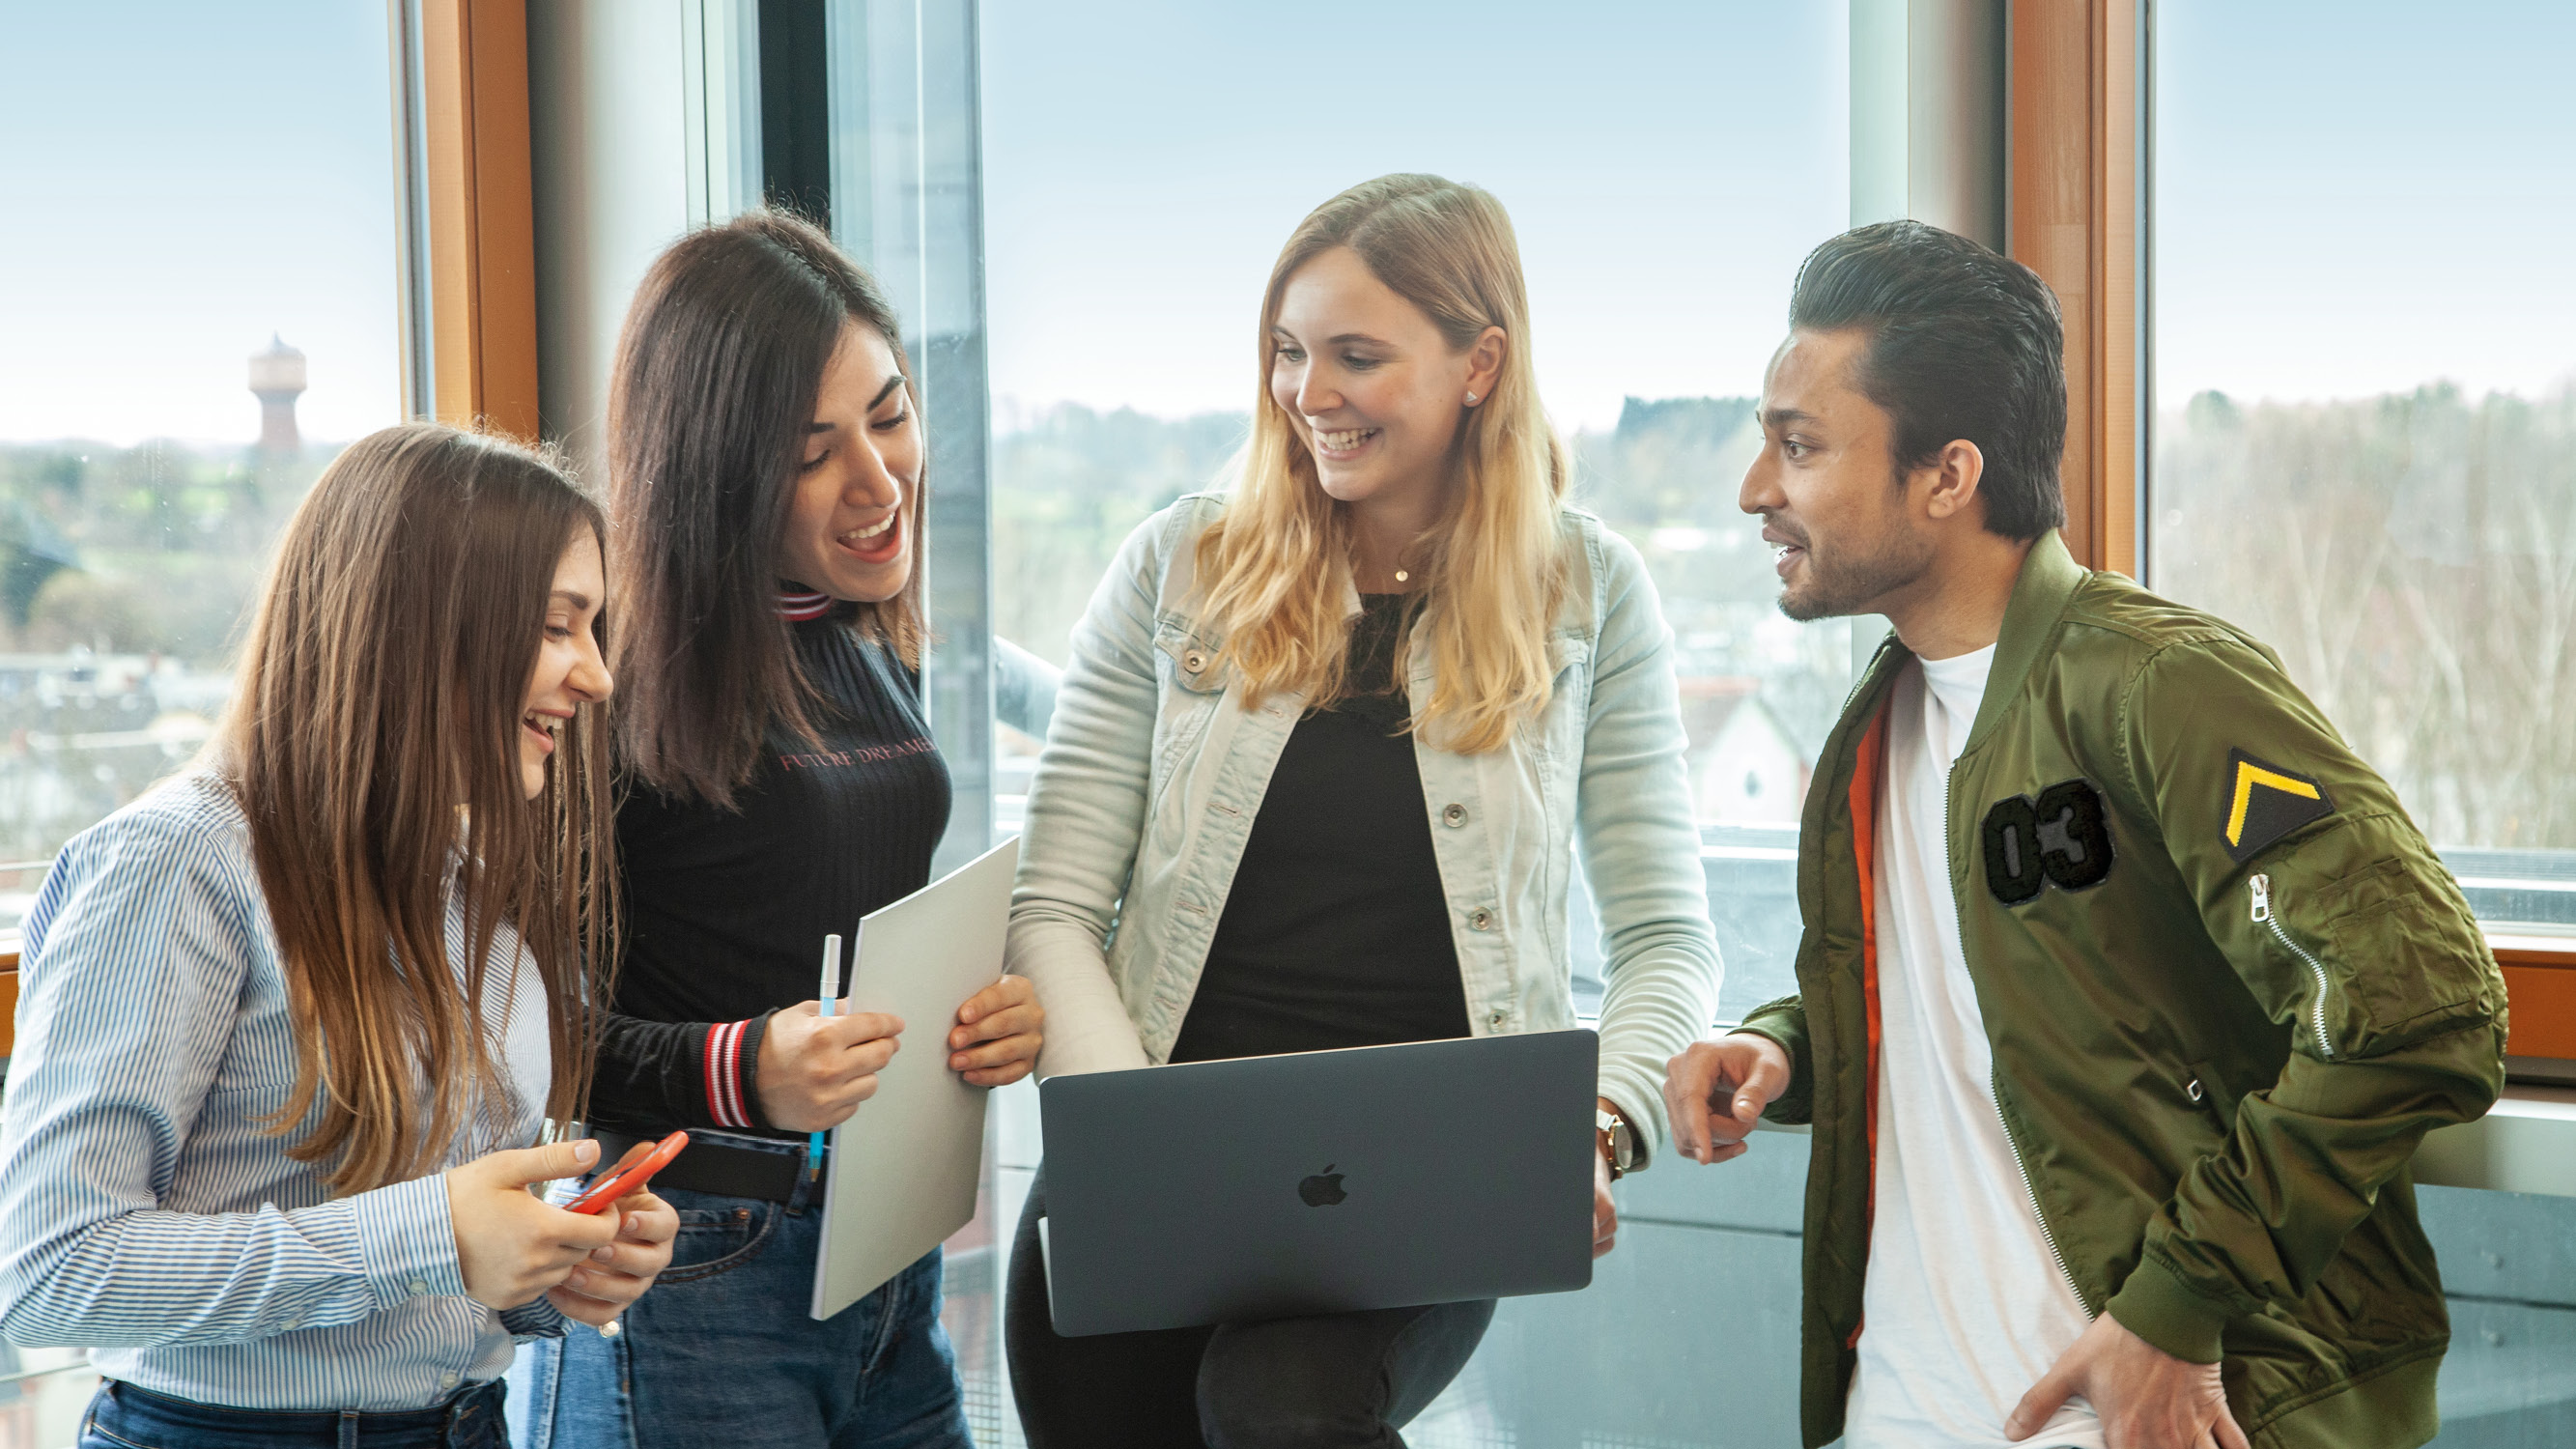
\includegraphics[width=\textwidth]{figures/thankyou.jpg}
				\captionof{figure}{Das Bild der Danke-Seite}
				\label{fig:thankyou}
			\end{column}
		\end{columns}
	\end{frame}

	\begin{frame}[fragile]{Inhalte absolut positionieren}
		\begin{itemize}
			\item Der Koordinatenursprung für ist die obere linke Ecke
			\item Koordinatensystem in Zentimetern, an Seitenverhältnis 16:9 ausgerichtet
			\begin{itemize}
				\item $ 0 \le x \le 16 $
				\item $ 0 \le y \le 9 $
			\end{itemize}

			\item Verwendung von \verb!begin{textblock}{breite}(x-pos, y-pos)!...
		\end{itemize}

		\begin{textblock}{5}(10, 4.5)
			\scriptsize
			\begin{verbatim}
				\begin{textblock}{5}(10, 4.5)
					Inhalt
				\end{textblock}
			\end{verbatim}
		\end{textblock}

		\begin{textblock}{15}(0.5, 6)
			\hrule
			\scriptsize
			\begin{verbatim}
				\begin{textblock}{15}(0.5, 6)
					\hrule
				\end{textblock}
			\end{verbatim}
		\end{textblock}
	\end{frame}

	\begin{frame} 
		\frametitle{Mehrere Folien mittels \textit{Overlays}} 
		\begin{theorem}
			Es gibt keine \enquote{größte} Primzahl.
		\end{theorem} 
		\begin{enumerate} 
			\item<1-| alert@1> Angenommen $p$ wäre die größte Primzahl.
			\item<2-> Sei $q$ das Produkt der ersten $p$ Zahlen. 
			\item<3-> Dann ist $q+1$ durch keine davon teilbar.
			\item<4-> Aber $q + 1$ ist größer als $1$ und daher durch eine Primzahl teilbar, die nicht in den ersten $p$ Zahlen liegt.
		\end{enumerate}

		\uncover<3->{\scriptsize Hinweis: Mathe ist super kompliziert!}

		\vfill
		\only<2,4>{\centering\textbf{Achtung}: Besonders wichtiger Schritt!}
		\vfill
	\end{frame}

	\section{Benutzerdefinierte Anpassungen}

	\newcommand{\rgb}[1]{\textcolor{hsmw80}{#1}}
	\newcommand{\cmd}[1]{\rgb{\textbackslash{}#1}}
	\newcommand{\textto}{\hspace*{0.2ex}\tikz[baseline=-.33em] \draw[-latex] (0,0) to ++(2ex, 0);\hspace*{0.2ex}}
	\begin{frame}{Zusätzliche, beeinflussbare Macros}{... und deren Abhängigkeiten (zur Feinabstimmung der eigenen Präsentation)}
		\begin{itemize}
			\item Option \rgb{hs}, \rgb{cb}, ... oder \rgb{faculty=cb, me, ...} (Farbschema)
			\begin{itemize}
				\item \cmd{insertfacultyicon} (Titelseite)
				\item \cmd{insertfacultyname} (Option \rgb{language}) \textto{} \cmd{institute\{\cmd{insertfacultyname}\}}
			\end{itemize}
			\item \cmd{insertthankyoutitle}, \cmd{insertthankyoutext}, \cmd{insertthankyousidebartext}
			\begin{itemize}
				\item \cmd{email} \textto{} \cmd{insertemail}
				\item \cmd{phone} \textto{} \cmd{insertmobilephone}, \cmd{inserttelephone}
				\item \cmd{office} \textto{} \cmd{insertoffice}
				\item \cmd{courseofstudies} \textto{} \cmd{insertcourseofstudies}
				\item \cmd{additional} \textto{} \cmd{insertadditionalsidebar}, \cmd{insertadditional}
			\end{itemize}
			\item \cmd{setcurrentspeaker}, \cmd{resetcurrentspeaker} (\cmd{insertshortauthor})
			\begin{itemize}
				\item Stern-Version (\cmd{setcurrentspeaker*}) setzt zusätzlich Label (Option \rgb{language})
				\item \cmd{currentspeaker} (\cmd{currentspeakerlabel}) \textto{} \cmd{insertcurrentspeaker}
			\end{itemize}
		\end{itemize}
	\end{frame}

	\section{FAQ}

	\begin{frame}[c]{FAQ: Häufig gestellte Fragen}{Hier ist noch Platz für Anwendungsfälle oder Antworten auf häufig gestellte Fragen}
		Es sind alle zum Testen und zur Übermittlung von konstruktivem Feedback eingeladen!
		\\[\baselineskip]
		Bei Ideen, Wünschen, Anregungen, Fragen und auch Problemen:
		\begin{itemize}
			\item Offizielle LaTeX-GitLab-Gruppe der Hochschule Mittweida:
			\newline
			\href{https://git.hs-mittweida.de/hsmw-latex}{git.hs-mittweida.de/hsmw-latex}

			\item Kontaktieren Sie mich gern per E-Mail \href{mailto:schildba@hs-mittweida.de?subject=[LaTeX] Beamer-Vorlage}{schildba@hs-mittweida.de}

			\item Nutzen Sie einen der anderen verfügbaren Kommunikationskanäle
		\end{itemize}
	\end{frame}

	\appendix
	\makebibliography
	\makethankyou

	\section{\appendixname}

	\begin{frame}{Zusätzliche Folien}{Der Anhang zählt nicht mit zu den regulären Folien}
		\blindtext
	\end{frame}

\end{document}
